%++++++++++++++++++++++++++++++++++++++++
% Don't modify this section unless you know what you're doing!
\documentclass[letterpaper,12pt]{article}
\usepackage{tabularx} % extra features for tabular environment
\usepackage{amsmath}  % improve math presentation
\usepackage{graphicx} % takes care of graphic including machinery
\usepackage[margin=1in,letterpaper]{geometry} % decreases margins
\usepackage{cite} % takes care of citations
\usepackage[final]{hyperref} % adds hyper links inside the generated pdf file
\usepackage{pgfplotstable, booktabs}
\usepackage{placeins}
\usepackage{tabularray}
\usepackage{titlesec}
\usepackage{fancyhdr}
\usepackage{empheq}
\usepackage{amssymb}
\usepackage{sectsty}
\usepackage{tcolorbox}
\usepackage{listings}
\usepackage{xcolor}
\usepackage{parskip}
\usepackage{cancel}
\usepackage{enumitem}
\usepackage{amsmath}
\usepackage{mathrsfs}
\usepackage{physics}
\usepackage{subcaption}
\usepackage{pdfpages}
\usepackage{amsthm} 

\definecolor{codegreen}{rgb}{0,0.6,0}
\definecolor{codegray}{rgb}{0.5,0.5,0.5}
\definecolor{codepurple}{rgb}{0.58,0,0.82}

\lstdefinestyle{mystyle}{
    commentstyle=\color{codegreen},
    keywordstyle=\color{codepurple},
    numberstyle=\tiny\color{codegray},
    stringstyle=\color{codegreen},
    basicstyle=\ttfamily\small,
    breakatwhitespace=false,         
    breaklines=true,                 
    captionpos=b,                    
    keepspaces=true,                                                     
    showspaces=false,                
    showstringspaces=false,
    showtabs=false,                  
    tabsize=4
}

\lstset{style=mystyle}
  
\newcommand*\widefbox[1]{\fbox{\hspace{0em}#1\hspace{0em}}}
\DeclareMathOperator{\Div}{div}
\DeclareMathOperator{\Grad}{grad}

\pagestyle{fancy}
\fancyhf{} % Clear all header and footer fields
\fancyhead[L]{MEC E 539}
%\fancyhead[C]{Center Header} 
\fancyhead[C]{Lecture Notes}
\fancyhead[R]{Alex Diep}

\fancyfoot[C]{\thepage}

\pgfplotsset{compat=1.18} 
\titleformat*{\section}{\Large\bfseries}
\titleformat*{\subsection}{\large\bfseries}

\renewcommand{\thesection}{Question \arabic{section}}
\renewcommand{\thesubsection}{(\alph{subsection})}
\renewcommand*{\arraystretch}{1.5}

\hypersetup{
	colorlinks=true,       % false: boxed links; true: colored links
	linkcolor=blue,        % color of internal links
	citecolor=blue,        % color of links to bibliography
	filecolor=magenta,     % color of file links
	urlcolor=blue         
}
%++++++++++++++++++++++++++++++++++++++++
\begin{document}
% \begin{titlepage}
%     \centering
%     \vspace*{2cm} % Adjust vertical spacing
    
%     % Title
%     \Huge {MEC E 301 \\Lab 1: Dimensional Measurement} \\
%     \vspace{1cm} % Adjust vertical spacing
    
%     % Author
%     \Large by: Alex Diep \\
%     \vspace{1cm} % Adjust vertical spacing

%     % Date
%     \Large Date: September 19, 2023 \\ % or manually specify a date
%     \vspace{4cm} % Adjust vertical spacing

%     % CCID and Student ID in smtaller font
%     \normalsize CCID: abdiep \\
%     \normalsize Student ID: 1664334 \\ 
%     \normalsize Section: D21 \\
    
%     \vfill % Fill vertical space
    
%     % Additional content (e.g., university logo or other information)
    
% \end{titlepage}

%\section*{Conservation of Energy (Scalar)}

Energy is a scalar quantity, and therefore it can be identified \& formulated through the conservation of a scalar quantity:

Let's try $\phi = $ scalar,
\begin{align*}
    \frac{\partial}{\partial t} \int_{\text{C.V.}} \rho \phi \, dV 
    + \int_{\text{C.S.}} \rho \phi (\vec{u} \cdot \vec{n}) \, dS &= 
    \oint_{\text{C.S.}} \Gamma \Grad(\phi) \cdot \vec{n} \, dS + 
    \int_{\text{C.V.}} \underbrace{q_{\phi}}_{\text{source/sink}} \, dV
\end{align*}

\begin{align*}
    \implies 
    \frac{\partial}{\partial t} (\rho \phi)  
    + \frac{\partial}{\partial x_j} (\rho \phi u_j) &=
    \frac{\partial}{\partial x_j} (\Gamma \frac{\partial \phi}{\partial x_j}) + q_{\phi}
\end{align*}
Conservation of a scalar (Energy). In vector notation,
\begin{align*}
    \partial_{t} (\rho \phi) + \Div (\rho \phi \vec{u}) &= 
    \Div (\Gamma \Grad (\phi)) + q_{\phi} 
\end{align*}
Where
\begin{itemize}
    \item $\partial_{t} (\rho \phi)$ is the time rate of change of the scalar quantity $\phi$ (conservative term).
    \item $\Div (\rho \phi \vec{u})$ is the rate of change due to the flow due to $\vec{u}$ (advection term).
    \item $\Div (\Gamma \Grad (\phi))$ is the rate of change due to diffusion ($\Gamma$) (diffusion term).
    \item $q_{\phi}$ is the rate of production (source) or destruction (sink) of $\phi$.
\end{itemize}

\section*{Chapter 4. Fundamental flows (Simplification)}
Navier-Stokes equations are highly non-linear PDEs with no exact solutions. However,
there are fundamental flow dynamics (simplified flows) based on assumptions and approximations that 
makes the mathematics easier to follow, solve, and interpret.

We are going to look at 4 simplified flow cases:
\begin{enumerate}
    \item Incompressible flow ($\rho = \text{constant}$)
    \item Invicid flow (Euler's flow) ($\mu \to 0$)
    \item Creeping flow (Stokes flow) ($\text{Re} \ll 100$, inertial forces are negligible)
    \item Potential flow ($\text{Re} \to 0$, $\text{Ma} \to 0$
\end{enumerate}
Let's look at the conservation laws for each:
\subsection*{Incompressible flow}
Incompressibility is defined as incapability of a fluid (i.e. liquid) to compress to a smaller size
under internal/external loads. This, therefore, means that their \textbf{density $\rho$} does
not change as long as we keep their mass the same.

Typically, liquids are incompressible, but air (gas) can become compressible at special conditions.
\[
 \underbrace{\text{Ma}}_{\vec{u} /\text{speed of sound}} > 0.3 \implies \text{compressible}
\]

Continuity:
\begin{align*}
    \cancelto{0 (\text{Incomp})}{\frac{\partial \rho}{\partial t}} + \divergence (\rho \vec{u}) &= 0 \\
    \implies \divergence \vec{u} &= 0
\end{align*}
Momentum:
\begin{align*}
    \frac{\partial}{\partial t} (\rho \vec{u}) + \divergence (\rho \vec{u} \vec{u}) &=
    - \grad P + \cancelto{0, \;\text{continuity}}{\frac{1}{3} \mu \nabla(\divergence \vec{u})} + \mu \laplacian \vec{u} + \rho \vec{b} \\
\end{align*}
Expanding the $\divergence (\rho \vec{u} \vec{u})$ term,
\begin{align*}
    \divergence (\rho \vec{u} \vec{u}) &= (\divergence \rho \vec{u}) \vec{u}
        + \rho \vec{u} \cdot \grad \vec{u} \\
    &= \cancelto{0, \;\text{continuity}}{(\divergence \rho \vec{u})} \vec{u}
        + \rho \vec{u} \cdot \grad \vec{u} \\
    &= \rho \vec{u} \cdot \grad \vec{u}
\end{align*}
Therefore,
\begin{align*}
    \frac{\partial}{\partial t} (\rho \vec{u}) + \rho \vec{u} \cdot \grad \vec{u} &=
    - \grad P + \mu \laplacian \vec{u} + \rho \vec{b} \\
    \rho \frac{\partial \vec{u}}{\partial t} + \rho \vec{u} \cdot \grad \vec{u} &=
    - \grad P + \mu \laplacian \vec{u} + \rho \vec{b} \\
    \frac{\partial \vec{u}}{\partial t} + \vec{u} \cdot \grad \vec{u} &=
    -\frac{\grad P}{\rho} + \underbrace{\frac{\mu}{\rho}}_{\nu} \laplacian \vec{u} + \vec{b} \\
\end{align*}

\subsection*{Invicid flow (Euler's flow)}
Viscous forces can be important in flows close to a wall, where we have large velocity gradients (Also in wakes).
As we should before, it is the combination of $\nu$ and $\vec{u}$ that forms the viscous effects in transport of fluids. 

$\implies$ Vorticies $\to$ $\nu$ may be important.

$\hookrightarrow$ if you are far from a surface or regions of large velocity gradients, the implication of viscocity becomes minimal.

$\hookrightarrow$ we quantify the effect of viscocity in the flow using Reynold's Number:
\begin{align*}
    \text{Re} = \frac{\rho u \overbrace{L}^{\text{characteristic length}}}{\mu} 
    = \frac{\text{inertial forces}}{\text{viscous forces}}
\end{align*}
if Re $\gg 1000 \implies \mu \to 0$ which means inertial forces dominate the flow 
(negligible viscous forces).

Continuity:
\begin{align*}
    \frac{\partial \rho}{\partial t} + \divergence (\rho \vec{u}) &= 0 
\end{align*}
No impact because no $\mu$ term.

Momentum:
\begin{align*}
    \frac{\partial}{\partial t} (\rho \vec{u}) + \divergence (\rho \vec{u} \vec{u}) &=
    - \grad P + \cancelto{0, \;\text{invicid}}{\frac{1}{3}\mu \nabla(\divergence \vec{u})}
    + \cancelto{}{\mu \laplacian \vec{u}} + \rho \vec{b} \\
\end{align*}
\begin{align*}
    \boxed{\frac{\partial}{\partial t} (\rho \vec{u}) + \divergence (\rho \vec{u} \vec{u}) =
    - \grad P + \rho \vec{b}}
\end{align*}
Note: As we saw in the Navier-Stokes equation, the flow can only be dominated by the 
\textbf{Pressure} and \textbf{External forces}. This means that the invicid cond. cannot hold if we 
are dealing with areas of high straining (vorcity and wakes).

Note: Since we are assuring invicid condition, then the flow cannot slow down close to the 
stationary wall. $\implies$ Slip Boundary Condition.

\subsection*{Creeping flow (Stokes flow)}
At high re, we just discussed that viscous effects are negligible. Contrarily, at low 
Re, (Re $\ll 100$) the effect of viscosity \textbf{dominates} the flow. 

$\implies$ Inertial forces are negligible.

\begin{align*}
    \text{Re} \propto \frac{u D}{\nu} 
    \begin{cases}
        \text{Either } u \to 0 \text{and/or} \\
        D \to 0 
    \end{cases}
\end{align*}

Continuity:
\begin{align*}
    \frac{\partial \rho}{\partial t} + \divergence (\rho \vec{u}) &= 0
\end{align*}
No impact.

Momentum:
\begin{align*}
    0 = - \frac{\grad P}{\rho} +  \divergence (\nu \grad \vec{u}) + \vec{b} + \vec{b}
\end{align*}
This type of flow is mostly for porous media coating, or nano-fluidics.

\subsection*{Potential flow}
One of the simpliest flows in fluid mechanics.

Based on two conditions:
\begin{enumerate}
    \item Invicid flow ($\mu \to 0$)
    \item Irrotational flow ($\vec{\omega} \to 0$)
\end{enumerate}
provides approximation for initial flow conditions.
\section*{Chapter 5: Non-Dimentionalization of the Flow}
Physically and mathematically, the flow results (dynamics) should not change based on the size of a simulation setup.

$\hookrightarrow$ Most fluid dynamics analyses are completed in a dimensionless framework. This allows for scaling of the real problem. 

$\hookrightarrow$ If the scaled conditions are maintained (i.e. Reynold's Number is the same), CFD simulations should be independent from geometrical or scalable physical parameters.

Note: The scalability of the flow condition holds only if the main flow behavior/dynamics is the same in terms of Re, $\rho$, $\mu$, \dots

Now, we return to our governing equations and discuss means to make them non-dimentionalized using normalization factors.

For example, velocity can be normalized using the freestream condition,
\begin{equation*}
    u_i = u_i^* u_{\infty} \implies u_i^* = \frac{u_i}{u_{\infty}}
\end{equation*}
where $u_{\infty}$ is the freestream velocity.

Similarly, 
\begin{equation*}
    t_0 = \frac{C}{u_{\infty}} \implies t^* = \frac{t}{t_0} = \frac{u_{\infty} t}{C}
\end{equation*}

For pressure,
\begin{equation*}
    P_{\text{dyn}} = \frac{1}{2} \rho u_{\infty}^2 \implies P^* = \frac{P}{P_{\text{dyn}}} = \frac{2 P}{\rho u_{\infty}^2}
\end{equation*}

and it is given that 
\begin{equation*}
    X_{i}^* = \frac{X_i}{C} \implies X_i = X_i^* C
\end{equation*}

$\hookrightarrow$ Now, let's begin with the continuity equation (incompressible)
\begin{align*}
    \frac{\partial u_i}{\partial x_i} &= 0 
\end{align*}
Substituting $u_i$ and $x_i$ with their non-dimensionalized counterparts,
\begin{align*}
    \frac{\partial u_i^* u_{\infty}}{\partial x_i^* C} &= 0 \\
    \cancel{\frac{u_{\infty}}{C}} \frac{\partial u_i^*}{\partial x_i^*} &= 0 \\
    \frac{\partial u_i^*}{\partial x_i^*} &= 0
\end{align*}

$\hookrightarrow$ Now, let's look at the momentum equation (incompressible)
\begin{align*}
    \frac{\partial u_i}{\partial t} + \frac{\partial (u_i u_j)}{\partial x_j} &= - \frac{1}{\rho} \frac{\partial P}{\partial x_i} + \nu \frac{\partial^2 u_i}{\partial x_j \partial x_j} + b_i
\end{align*}
Then,
\begin{align*}
    \frac{\partial (u_i^* u_{\infty})}{\partial (t^* t_0)} + \frac{\partial (u_i^* u_j^* u_{\infty}^2)}{\partial (x_j^* C)} 
    &= - \frac{1}{\rho} \frac{\partial (P^* P_{\text{dyn}})}{\partial (x_i^* C)} + \nu \frac{\partial^2 (u_i^* u_{\infty})}{\partial (x_j^* C) \partial (x_j^* C)} + g b_i^* \\
    \frac{\partial (u_i^* u_{\infty})}{\partial (t^* t_0)} + \frac{\partial (u_i^* u_j^* u_{\infty}^2)}{\partial (x_j^* C)}
    &= - \frac{1}{\rho} \frac{\partial (P^* P_{\text{dyn}})}{\partial (x_i^* C)} + \nu \frac{\partial^2 (u_i^* u_{\infty})}{\partial (x_j^* C) \partial (x_j^* C)} + g b_i^* \\
    \left(\frac{u_{\infty}}{t_0}\right) \frac{\partial u_i^*}{\partial t^*} + \left(\frac{u_{\infty}^2}{C}\right) \frac{\partial (u_i^* u_j^*)}{\partial x_j^*}
    &= - \frac{1}{\rho} \left(\frac{\frac{1}{2}\rho u_{\infty}^2}{C}\right) \frac{\partial P^*}{\partial x_i^*} + \left(\frac{\nu u_{\infty}}{C^2}\right) \frac{\partial^2 u_i^*}{\partial x_j^* \partial x_j^*} + g b_i^* 
\end{align*}
Now multiply by $C/u_{\infty}^2$,
\begin{align*}
    \frac{C}{u_\infty t_0}\frac{\partial u_i^*}{\partial t^*} + \frac{\partial (u_i^* u_j^*)}{\partial x_j^*}
    &= - \frac{1}{2} \frac{\partial P^*}{\partial x_i} + \frac{\nu}{u_{\infty} C} \frac{\partial^2 u_i^*}{(\partial x_j^*)^2} + \frac{g C}{u_{\infty}^2} b_i^*
\end{align*}
Therefore we obtain a number of important characteristic flow quantities:
\begin{enumerate}
    \item Strouhal Number: This dimentionless number is wkd as a number to describe flow unsteadiness (periodicity). Hence, $f_i = 1/t_i$ in the frequency of unsteadiness, which relates to vortex formulation frequency, flapping wings, etc.
    \begin{equation*}
        \text{St} = \frac{f_i C}{u_{\infty}} = \frac{C}{\underbrace{P_i}_{\text{Period}} u_{\infty}}
    \end{equation*}
    \item Reynold's Number: Describes the ratio of inertial to viscous effects.
    \begin{equation*}
        \text{Re} = \frac{\rho u_{\infty} C}{\mu} = \frac{u_{\infty} C}{\nu}
    \end{equation*}
    \item Froude Number: Describes the ratio of inertial to external fields in the flow
    \begin{equation*}
        \text{Fr} = \frac{u_{\infty}}{\sqrt{Cg}}
    \end{equation*}
    This enables us to understand if the flow is driven by inertial forces or external effects (gravity)
\end{enumerate}
From the energy equation, we will get the Peclet Number, which describes the ratio of convection to diffusion effects.
\begin{equation*}
    \text{Pe} = \frac{C u_{\infty}}{k/\rho C_p}
\end{equation*}


 %questions for after class
    %1. what happened to the time term in the inviscid continuity equation?
<<<<<<< HEAD
\subsection*{Boundary Layer Approximation}
Boundary layers are one of the most common fluid flow phenomena observed in nature. In fact, the wind on an Earth's atmosphere is the result of a boundary layer developed by moving air next to the planet's surface. This is referred to as the atmospheric boundary.
$\hookrightarrow$ Correct understanding of the flow dynamics inside the boundary layer is critical in technology development, control systems, and weather forecasting. 

In classical fluid mechanics, we make unique assumptions, based in which we can apply certain approximating to our governing equations. For a laminar boundary layer, there are 3 assumption that drive our approximation process.
\begin{enumerate}
    \item B.L are 2-D. $\implies$ at high Re, this can become problematic.
    \item The thickness of the B.L. ($\delta$) is small compared to the other characteristic length. $\implies$ Mostly true.
    \item The flow velocity in the streamwise direction dominates. $\implies$ Provable.
\end{enumerate}
\begin{figure}
    \centering
    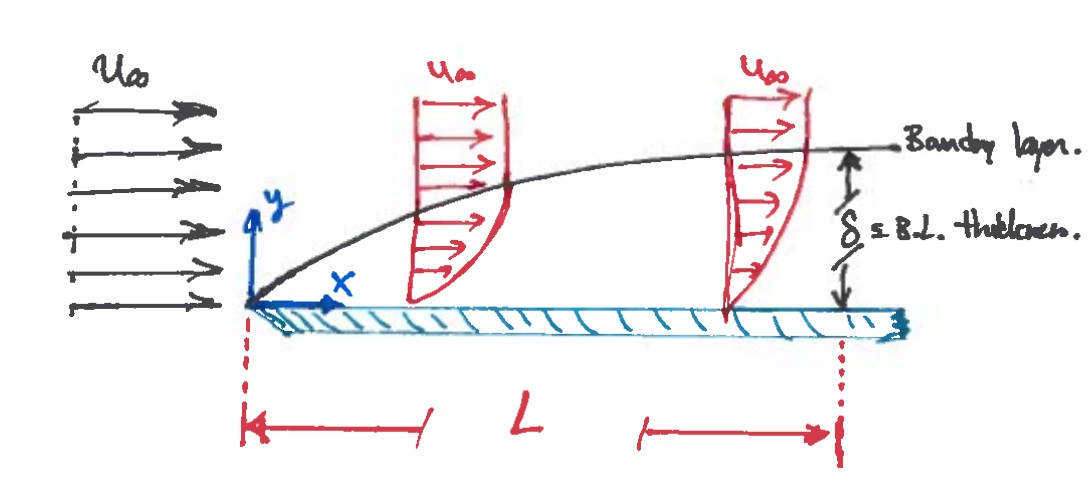
\includegraphics[width=0.5\linewidth]{Lecture Number/Figures/Lecture 6, Jan 30, 2024, Boundary Layer Concept.jpg}
    \caption{Boundary Layer Concept}
    \label{fig:Boundary Layer Concept}
\end{figure}
Assuming that Re$_{l} \gg 1$ and $\delta \ll \ell$, then we can rely on the following normalization factors (order of magnitude analysis).
\begin{table}
    \centering
    \caption{Order of Magnitude Analysis}
    \label{tab:Order of Magnitude Analysis}
    \begin{tabular}{c|ccc}
        & \textbf{Variable} & \textbf{Order of Magnitude} & \textbf{Normalization Factor} \\
        \hline
        Streamline Velocity & $u$ & $u_{\infty}$ & $u = u^* u_{\infty}$ \\
        Streamline Spatial Coordinate & $x$ & $\ell$ & $x = x^* \ell$ \\
        Orthogonal Directional Coordinate & $y$ & $\delta$ & $y = y* \delta$ \\
        Orthogonal Velocity & $v$ & $\mathcal{V}$?? & $v = v* \mathcal{V}$ \\
        \end{tabular}
\end{table}
Let's start with the continuity equation (incompressible flow):
\begin{gather*}
    \frac{\partial u_i}{\partial x_i} = 0 \\
    \frac{\partial u}{\partial x} + \frac{\partial v}{\partial y} = 0 \\
    \frac{\partial u^* u_{\infty}}{\partial x^* \ell} + \frac{\partial v^* \mathcal{V}}{\partial y^* \delta} = 0 \\
    \implies \left(\frac{u_{\infty}}{\ell}\right) \frac{\partial u^*}{\partial x^*} + \left(\frac{\mathcal{V}}{\delta}\right) \frac{\partial v^*}{\partial y^*} = 0 \\
    \implies \frac{\partial u^*}{\partial x^*} +\frac{\mathcal{V} \ell}{u_{\infty} \delta} \frac{\partial v^*}{\partial y^*} = 0 \\
\end{gather*}
Based on the order of magnitude analysis, 
\begin{gather*}
    \frac{\mathcal{V} \ell}{u_{\infty} \delta} = 1 \\
    \implies \mathcal{V} = \frac{u_{\infty} \delta}{\ell} \\
\end{gather*}
Therefore, if $\delta ll \ell$, then $\mathcal{V} \ll u_{\infty}$. This provies that streamline velocity dominates. 

Now, let's move to the Navier-Stokes equation. First, the x-dir:
\begin{gather*}
    \cancelto{\frac{\partial u}{\partial t}}{\text{S.S.}} + u \frac{\partial u}{\partial x} + v \frac{\partial u}{\partial y} = -\frac{1}{\rho} \frac{\partial P}{\partial x} + \nu \left(\frac{\partial^2 u}{\partial x^2} + \frac{\partial^2 u}{\partial y^2}\right) 
\end{gather*}
y-dir:
\begin{gather*}
    \cancelto{\frac{\partial v}{\partial t}}{\text{S.S.}} + u \frac{\partial v}{\partial x} + v \frac{\partial v}{\partial y} = -\frac{1}{\rho} \frac{\partial P}{\partial y} + \nu \left(\frac{\partial^2 v}{\partial x^2} + \frac{\partial^2 v}{\partial y^2}\right)
\end{gather*}

Let's look at the x-dir expression:
\begin{gather*}
    (u^* u_{\infty}) \frac{\partial (u^* u_{\infty})}{\partial (x^* \ell)} + (v^* \mathcal{V}) \frac{\partial (u^* u_{\infty})}{\partial (y^* \delta)} = -\frac{1}{\rho} \frac{\partial P}{\partial (x^* \ell)} + \nu \left(\frac{\partial^2 (u^* u_{\infty})}{\partial (x^* \ell)^2} + \frac{\partial^2 (u^* u_{\infty})}{\partial (y^* \delta)^2}\right) \\
    %---------------------------------------
    \implies \left(\frac{u_{\infty}^2}{\ell}\right) u^* \frac{\partial u^*}{\partial x^*} + \left(\frac{u_{\infty} \mathcal{V}}{\delta}\right) v^* \frac{\partial u^*}{\partial y^*} = -\frac{1}{\rho \ell} \frac{\partial P}{\partial x^*} + \nu \left(\left(\frac{u_{\infty}}{\ell^2}\right) \left(\frac{\partial^2 u^*}{\partial (x^*)^2} + \left(\frac{u_{\infty}}{\delta^2}\right) \frac{\partial^2 u^*}{\partial (y^*)^2}\right)\right) 
\end{gather*}
Using $\mathcal{V} = \frac{u_{\infty} \delta}{\ell}$, 
\begin{gather*}
    \left(\frac{u_{\infty}^2}{\ell}\right) u^* \frac{\partial u^*}{\partial x^*} + \left(\frac{u_{\infty}^2}{\ell}\right) v^* \frac{\partial u^*}{\partial y^*} = -\frac{1}{\rho \ell} \frac{\partial P}{\partial x^*} + \frac{\nu u_{\infty}}{\delta^2} \left(\cancelto{\left(\frac{\delta^2}{\ell^2}\right)}{0} \frac{\partial^2 u^*}{\partial (x^*)^2} + \frac{\partial^2 u^*}{\partial (y^*)^2}\right) 
\end{gather*}
Note the term inside the $\nu$ term is zero since $\delta \ll \ell$. From order of magnitude analysis, we can say
\begin{equation*}
    \text{Scaling of LHS} ~ \text{Scaling of RHS}
\end{equation*}
% i missed this part
% \begin{gather*}
%     \frac{u_{\infty}^2}{\ell} \sim \frac
\begin{gather*}
    \frac{\delta^2}{\ell^2} ~ \frac{\nu}{\ell u_{\infty}} = \frac{1}{\text{Re}}
\end{gather*}
So, if $\delta^2 \ll \ell^2$, then $\frac{1}{\text{Re}} \ll 1$. This implies the flow remains 2D for high Re. 

At this point, we can look at the scaling for pressure,
\begin{gather*}
    \frac{u_{\infty}^2}{\ell} ~ (\text{Pressure Scaling}) \left(\frac{1}{\rho}
    \frac{\partial P}{\partial x} = 0 \left(\frac{\rho u_{\infty}^2}{\ell}\right)\right)
\end{gather*}
Let's apply the same process to the y-direction. The results are:
\begin{gather*}
    \left(\frac{u_{\infty} \mathcal{V}}{\ell}\right) u^* \frac{\partial v^*}{\partial x^*} + \left(\frac{\mathcal{V}^2}{\delta^2}\right) v^* \frac{\partial v^*}{\partial y^*} = -\frac{1}{\rho} \frac{\partial P}{\partial y} + \nu \left(\left(\frac{\mathcal{V}}{\ell^2}\right) \frac{\partial^2 v^*}{\partial (x^*)^2} + \left(\frac{\mathcal{V}}{\delta^2}\right) \frac{\partial^2 v^*}{\partial (y^*)^2}\right) 
\end{gather*}
Since $\delta/\ell \ll 1$ and $u_{\infty} \mathcal{V}/\ell = 0$
\begin{gather*}
    \implies 0 = \frac{1}{\rho} \frac{\partial P}{\partial y^*} 
\end{gather*}
We can see that 
\begin{gather*}
    \text{Scaling of } \frac{\partial P}{\partial y} ~ \frac{u_{\infty}^2 \delta}{\ell^2} \\
    % \frac{\partial P}{\partial x} ~ \rho \frac{\u_{\infty}^2}{\ell} 
\end{gather*}
We can again show that 
\begin{gather*}
    \frac{\partial P}{\partial x} gg \frac{\partial P}{\partial y} 
\end{gather*}
=======
>>>>>>> 0a5eda1587e4060abce25b38456719d4f931cab4
% \newpage
% %\bibliographystyle{IEEEtran}
% %\bibliography{citations.bib}
% %\bibliography{}

% \newpage
% \appendix
% \section{Appendix: Arduino Uno Accuracy}
\label{sec:appendix-arduino-accuracy}
Table \ref{tab:arduino-accuracy-appendix} summarizes the range, resolution, repeatability, accuracy, and manufacturer's accuracy for various ranges of the 
Arduino Uno. Sample calculations for the 5V reference voltage are shown below. Note, the manufacturer's accuracy is $\pm$ 2 LSBs.

\begin{align*}
    \text{Resolution} &= \frac{V_{\text{ru}} - V_{\text{rl}}}{2^n} \\
    &= \frac{5.000 - 0.000}{2^{10}} \\
    &= \boxed{\qty[per-mode=symbol]{4.883}{\milli\volt\per\LSB}} \\
    \text{Repeatability} &= \max({\text{Max Deviation}}) \\
    &= \max(\langle 5.00, 0.00, 9.00, 44.00 \rangle) \\
    &= \boxed{\qty{44.00}{\milli\volt}} \\
    \text{Accuracy} &= \max({\text{Deviation}}) \\
    &= \max\left(
        \tiny	
        \begin{bmatrix}
            -0.009 & -0.009 & -0.009 & -0.009 & -0.009 & -0.009 & -0.009 & -0.009 & -0.004 & -0.009 \\
            0.001 & 0.001 & 0.001 & 0.001 & 0.001 & 0.001 & 0.001 & 0.001 & 0.001 & 0.001 \\
            0.016 & 0.021 & 0.012 & 0.016 & 0.012 & 0.012 & 0.016 & 0.016 & 0.012 & 0.016 \\
            0.02 & 0.024 & 0.02 & 0.024 & 0.01 & 0.02 & \textbf{0.054} & 0.024 & 0.034 & 0.02 \\
        \end{bmatrix}
    \right) \nonumber \\
    &= \boxed{\qty{54.00}{\milli\volt}}\\
    \text{Manuf. Acc.} &= \qty{2}{\LSB} \times \text{Resolution} \\
    &= \boxed{\qty{9.766}{\milli\volt}}
\end{align*}

\noindent For significant figures, since the range is given to 3 decimal places, the resolution is given to 3 decimal places, more often
than not, the number of significant figures is 4. This is because addition and subtraction do not take into account the number of significant figures
but rather the number of decimal places.

\begin{table}[ht]
    \caption{Range, Resolution, Repeatability, Accuracy, and Manufacturer's Accuracy for Various Ranges of the Arduino Uno}
    \label{tab:arduino-accuracy-appendix}
    \centering
    \small
    \begin{tabular}{lccccc}
        \toprule
        Arduino Config. & Range & Resolution & Repeatability & Acc. & Manuf. Acc. \\
        & (V) & (mV/LSB) & (mV) & (mV) & (mV) \\
        \midrule
        5V Ref. & 0.000 - 5.000 & 4.883 & 44.00 & 54.00 & 9.766 \\
        3.3V Ref. & 0.000 - 3.300 & 3.223 & 4.000 & 17.00 & 6.445 \\
        3.3V Ref., 10x VDiv & 0.00 - 33.00 & 32.23 & 32.00 & 83.00 & 64.45 \\
        3.3V Ref., [-10, 10]V & -10.00 - 10.00 & 19.53 & 0.000 & 24.00 & 39.06 \\
        3.3V Ref., 10x Amp. & 0.000 - 0.330 & 0.3223 & 0.000 & 0.000 & 0.6445 \\
        \bottomrule
    \end{tabular}
\end{table}

\FloatBarrier
\phantom{a}
\end{document}